\chapter{Observatorios y colaboraciones que usan WCD's}\label{OBSERVATORIOS_COLABORACIONES}
\section{Observatorios}
	\subsection{LHAASO (The Large High Altitude Air Shower Observatory)}\label{LHAASO}
	El observatorio LHAASO se construirá en China, provincia de Sichuan, a una altura de 4400 m.s.n.m., el arreglo completo incluye alrededor de 1171 detectores de muones con el objetivo de estudiar y entender mejor las fuentes de los rayos cósmicos ultra-energéticos, por lo que su rango de energía en el cual se enfoca es desde los $10^{13}-10^{18} eV$. LHAASO tiene un area de detección de $40000 m^{2}$ donde de colocarán las unidades MD (muon detector). Dentro de los tanques (altura de 1,2 m y diámetro de 6,8 ) se coloca un material altamente reflectante y un tubo fotomultiplicador de 8 pulgadas \cite{ZUO20181}.
	
	\subsection{HAWC (High Altitude Water Cherenkov)}\label{HAWC}
	El observatorio de rayos gamma HAWC se encuentra situado en Sierra Negra, Mexico a aproximadamente 4100 msnm. HAWC es una colaboración internacional en la cual participan más de 30 investigadores de Mexico y EEUU con el objetivo de detectar rayos gamma con energía de entre 100 GeV y 100 TeV y con ello extender nuestro conocimiento de las fuentes cósmicas de los rayos gamma \cite{Bonilla}.
	
	\subsection{Pierre Auger}\label{PIERRE_AUGER}
	Construido en la provincia de Mendoza, Argentina, el Observatorio Pierre Auger es el observatorio más grande actualmente para medir rayos cósmicos de energía ultra alta con energías de hasta $10^{18} $eV. Este observatorio utiliza dos tipos de detectores: el primero es de superficie o detector Cherenkov de Agua (WCD), ver fig.~\ref{TANQUE_PIERRE_AUGER}, cuya finalidad es de reconstruir el desarrollo lateral de las lluvias por medio de la detección de partículas que llega al detector. El segundo son los telescopios de fluorescencia que son utilizados para el estudio de la longitud de desarrollo de las lluvias \cite{A.C.Cobos}.

	\begin{figure}[h]
		\centering
		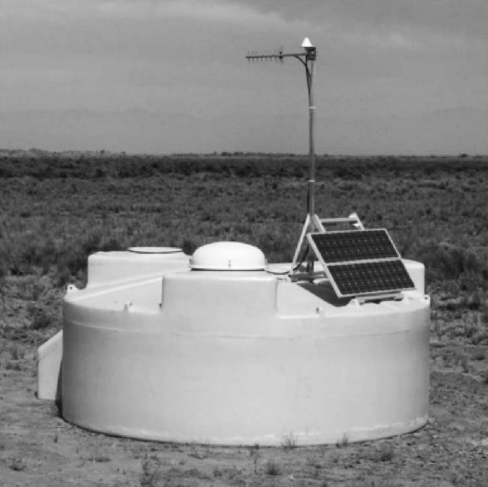
\includegraphics[scale=0.6]{FIGURAS/TANQUE_PIERRE_AUGER.PNG}
		\caption{Una estación de detacción instalada en el Observatorio Pierre Auger}
		\label{TANQUE_PIERRE_AUGER}
	\end{figure}

\section{Colaboraciones SWGO y LAGO}
	\subsection{Colaboración SWGO (Southern Wide-field Gamma-ray Observatory)}\label{SWGO}
	La detección de rayos gamma y CR han demostrado un importante potencial científico gracias a los observatorios de HAWC y LHAASO. Sin embargo, estos operan observando el hemisferio norte, por lo que la colaboración SWGO pretende ampliar ese campo de visión y mapeo del universo hacia el hemisferio sur, ver fig. \ref{MAPEO_SWGO}, construyendo observatorios que usen la tecnología de los WCD. El acceso al centro galáctico y el trabajo complementario con el observatorio CTA-Sur forman también parte de sus motivaciones para la construcción de un observatorio en el hemisferio sur \cite{schoorlemmer2019nextgeneration}. Una de las condiciones de SWGO para la construcción de un observatorio es que el lugar este situado a gran altitud, por lo que ciertas partes partes de la región Arequipa, Perú representan lugares prometedores para un futuro observatorio. Por otro lado SWGO tiene una red amplia de colaboradores alrededor del mundo, entre ellos se encuentra Perú, bajo la dirección y representación del Dr. José Bellido Cáceres, y la Universidad Nacional de San Agustín de Arequipa.
	
	\begin{figure}[h]
		\centering
		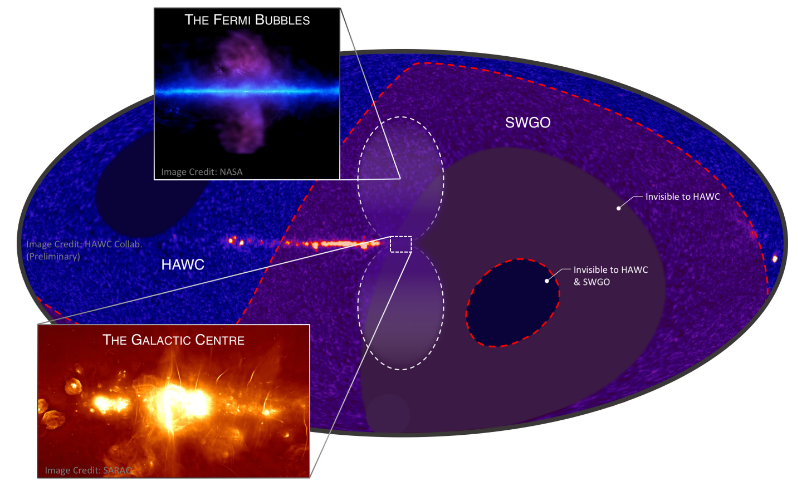
\includegraphics[scale = 0.45]{FIGURAS/MAPEO_SWGO.png}
		\caption{Mapeo que pretende realizar la colaboración SWGO (zona sombreada de rojo) mediante la construcción de un observatorio en el hemisferio sur \cite{schoorlemmer2019nextgeneration}.}
		\label{MAPEO_SWGO}
	\end{figure}
	
	\subsection{Colaboración LAGO (Latin American Giant Observatory)}\label{LAGO}
	La colaboración LAGO es un observatorio compuesto por una red de WCD's distribuidos por toda latino-américa, es decir, WCD's situados en diferentes lugares a diferentes altitudes, desde el nivel del mar hasta 5000 msnm. Los detectores de LAGO pueden contener de 1 a 40m$^3$ de agua purificada. Este observatorio esta diseñado para medir la evolución temporal del flujo de rayos cósmicos provinientes del espacio exterior evaluando tres aspectos: fenómenos de alta energía, clima espacial y radiación atmosférica a nivel del suelo. LAGO es entonces, una colaboración descentralizada que se expande desde el sur de México hasta la Patagonia gracias a la colaboración de más de 30 instituciones de 10 paises \cite{SIDELNIK2017173}. Para el desarrollo de la presente actividad se trabajó con datos compartidos por el proyecto LAGO, buscando los protocolos de calibración para estos detectores.
	
	